\documentclass[10pt,twocolumn]{article}
\usepackage{times}
\usepackage[margin=0.75in,top=1in]{geometry}
\usepackage{graphicx}
\usepackage{booktabs}
\usepackage{amsmath}
\usepackage{amssymb}
\usepackage{hyperref}
\usepackage{microtype}
\usepackage{xcolor}
\usepackage{caption}
\usepackage{subcaption}
\usepackage{enumitem}
\usepackage{tikz}
\usetikzlibrary{shapes.geometric, arrows.meta, positioning, fit, backgrounds}

\setlength{\columnsep}{0.25in}

\title{\textbf{Parameter-Efficient Fine-Tuning of MobileSAM\\
with LoRA for Nuclei Instance Segmentation}}

\author{
  Taiwo Olabamipe \\
  Computer Science \\
  University of Central Florida \\
  CAP5516 -- Assignment 3 \\
  \texttt{tal17847@ucf.edu}
}

\date{}

\begin{document}

\maketitle

% ----------------------------------------------------------------
\begin{abstract}
\textit{
We present a parameter-efficient fine-tuning framework for nuclei
instance segmentation in H\&E-stained histological images.
MobileSAM~\cite{zhang2023mobilesam}, a lightweight variant of the
Segment Anything Model (SAM)~\cite{kirillov2023sam}, is adapted
to the NuInsSeg dataset~\cite{mahbod2024nuinsseg} using Low-Rank
Adaptation (LoRA)~\cite{hu2021lora} injected into the query and
value projection matrices of TinyViT's self-attention blocks,
while the mask decoder is fully fine-tuned. Only \textbf{4.12M
parameters} (40.4\% of the 10.2M total) are trained. Training
follows a five-fold cross-validation protocol across the full
NuInsSeg dataset (674 images, 23 tissue types), using paired
positive--negative centroid point prompts derived from ground-truth
instance maps. The combined per-instance Dice and focal loss is
augmented with an auxiliary IoU prediction loss to improve mask
confidence calibration. Our method achieves mean
Dice\,=\,0.9085, AJI\,=\,0.7459, and PQ\,=\,0.7459, with
notably low cross-fold variance (AJI std\,=\,0.0028).
}

\medskip
Source code: \url{https://github.com/olabamipetaiwo/Segmentation}
\end{abstract}
% ----------------------------------------------------------------

\section{Introduction}

Nuclei instance segmentation in histopathology images is a
fundamental step in computational pathology pipelines, enabling
downstream tasks such as tumour grading, cell counting, and
biomarker quantification. The NuInsSeg dataset~\cite{mahbod2024nuinsseg}
provides fully annotated H\&E images from 31 human and mouse
organs, challenging models to segment individual nuclei across
diverse tissue types with varying staining protocols and cell
densities.

Foundation models for image segmentation, led by
SAM~\cite{kirillov2023sam}, achieve remarkable zero-shot
generalisation across natural images but require adaptation for
medical imaging domains, where appearance statistics differ
significantly from natural images~\cite{mazurowski2023sam}.
Vanilla fine-tuning of large vision models is impractical when
only tens to hundreds of annotated images are available; it risks
catastrophic forgetting and is computationally expensive.

LoRA~\cite{hu2021lora} addresses this by introducing trainable
low-rank matrices in parallel to frozen weight matrices, enabling
effective domain adaptation with a small fraction of trainable
parameters. Applied to attention layers, LoRA has proven
competitive with full fine-tuning across vision and language
tasks while preserving the learned representations of the
backbone~\cite{hu2021lora}.

This work applies LoRA to the image encoder of
MobileSAM~\cite{zhang2023mobilesam} --- a lightweight SAM
variant that distils ViT-H into a TinyViT encoder 50$\times$
faster at inference --- and fine-tunes the mask decoder for
nuclei instance segmentation on NuInsSeg. We report 5-fold
cross-validation metrics (Dice, AJI, PQ) across 23 human
tissue types and analyse the gap between prompt-assisted and
fully automatic inference.

\section{Methodology}

\subsection{Dataset}

NuInsSeg~\cite{mahbod2024nuinsseg} contains 665 image patches
(512$\times$512~px) from 31 tissue types, with expert-annotated
nuclei polygon masks for every nucleus. We train and evaluate on
the full human tissue subset of NuInsSeg (674 images across 23
tissue types including muscle, kidney, liver, lung, brain, and
others), using five-fold cross-validation splits (539 train /
135 val per fold). Ground-truth instance maps (uint16 TIF files)
are loaded directly; binary masks and distance maps are derived
from them using SciPy's Euclidean distance transform.

\subsection{Model Architecture}

\textbf{MobileSAM overview.}
MobileSAM~\cite{zhang2023mobilesam} replaces SAM's heavyweight
ViT-H image encoder with TinyViT~\cite{wu2022tinyvit}, a 5M-parameter
hierarchical vision transformer distilled from ViT-H. Like SAM,
it consists of three components: (1)~an \emph{image encoder}
(TinyViT) that maps a 1024$\times$1024 RGB image to a
$64\times64\times256$ feature embedding; (2)~a \emph{prompt
encoder} that converts point, box, or mask prompts to sparse
or dense embeddings; and (3)~a \emph{mask decoder} that cross-attends
image and prompt embeddings to produce segmentation masks and
IoU confidence scores.

\textbf{LoRA injection.}
TinyViT's self-attention blocks use a fused projection
$\mathbf{W}_{QKV} \in \mathbb{R}^{d \times 3d}$ for computational
efficiency. We decompose this into three separate projections
and inject LoRA adaptors into the query (\textbf{Q}) and value
(\textbf{V}) streams only, leaving the key (\textbf{K})
stream frozen --- following the design of SAMed~\cite{zhang2023samed}
which showed this decomposition is sufficient. For each target
projection $\mathbf{W} \in \mathbb{R}^{d_{in} \times d_{out}}$:

\begin{equation}
  \mathbf{W}' = \mathbf{W} + \frac{\alpha}{r}\,\mathbf{B}\mathbf{A},
  \qquad
  \mathbf{A} \in \mathbb{R}^{r \times d_{in}},\;
  \mathbf{B} \in \mathbb{R}^{d_{out} \times r}
\end{equation}

where $r = 8$ is the LoRA rank, $\alpha = 1.0$ is the scaling
factor, $\mathbf{A}$ is initialised with Kaiming uniform noise,
and $\mathbf{B}$ with zeros (so $\Delta\mathbf{W}=0$ at
initialisation). LoRA adaptors are added to all attention
blocks in TinyViT layers~1--4, yielding 40~trainable LoRA
tensors in total (10~blocks $\times$ 2~projections $\times$
2~matrices).

\textbf{Trainable parameter breakdown.}

\begin{center}
\small
\begin{tabular}{lr}
\toprule
\textbf{Component} & \textbf{Parameters} \\
\midrule
LoRA (rank 8, Q \& V)  & 59,392 \\
Mask Decoder (fully unfrozen) & 4,058,340 \\
\midrule
\textbf{Total Trainable} & \textbf{4,117,732} \\
Frozen (image encoder backbone) & 6,071,752 \\
\midrule
Total Model & 10,189,484 \\
\textbf{Trainable \%} & \textbf{40.4\%} \\
\bottomrule
\end{tabular}
\end{center}

Figure~\ref{fig:arch} illustrates where LoRA layers sit within
the overall pipeline.

\begin{figure*}[t]
\centering
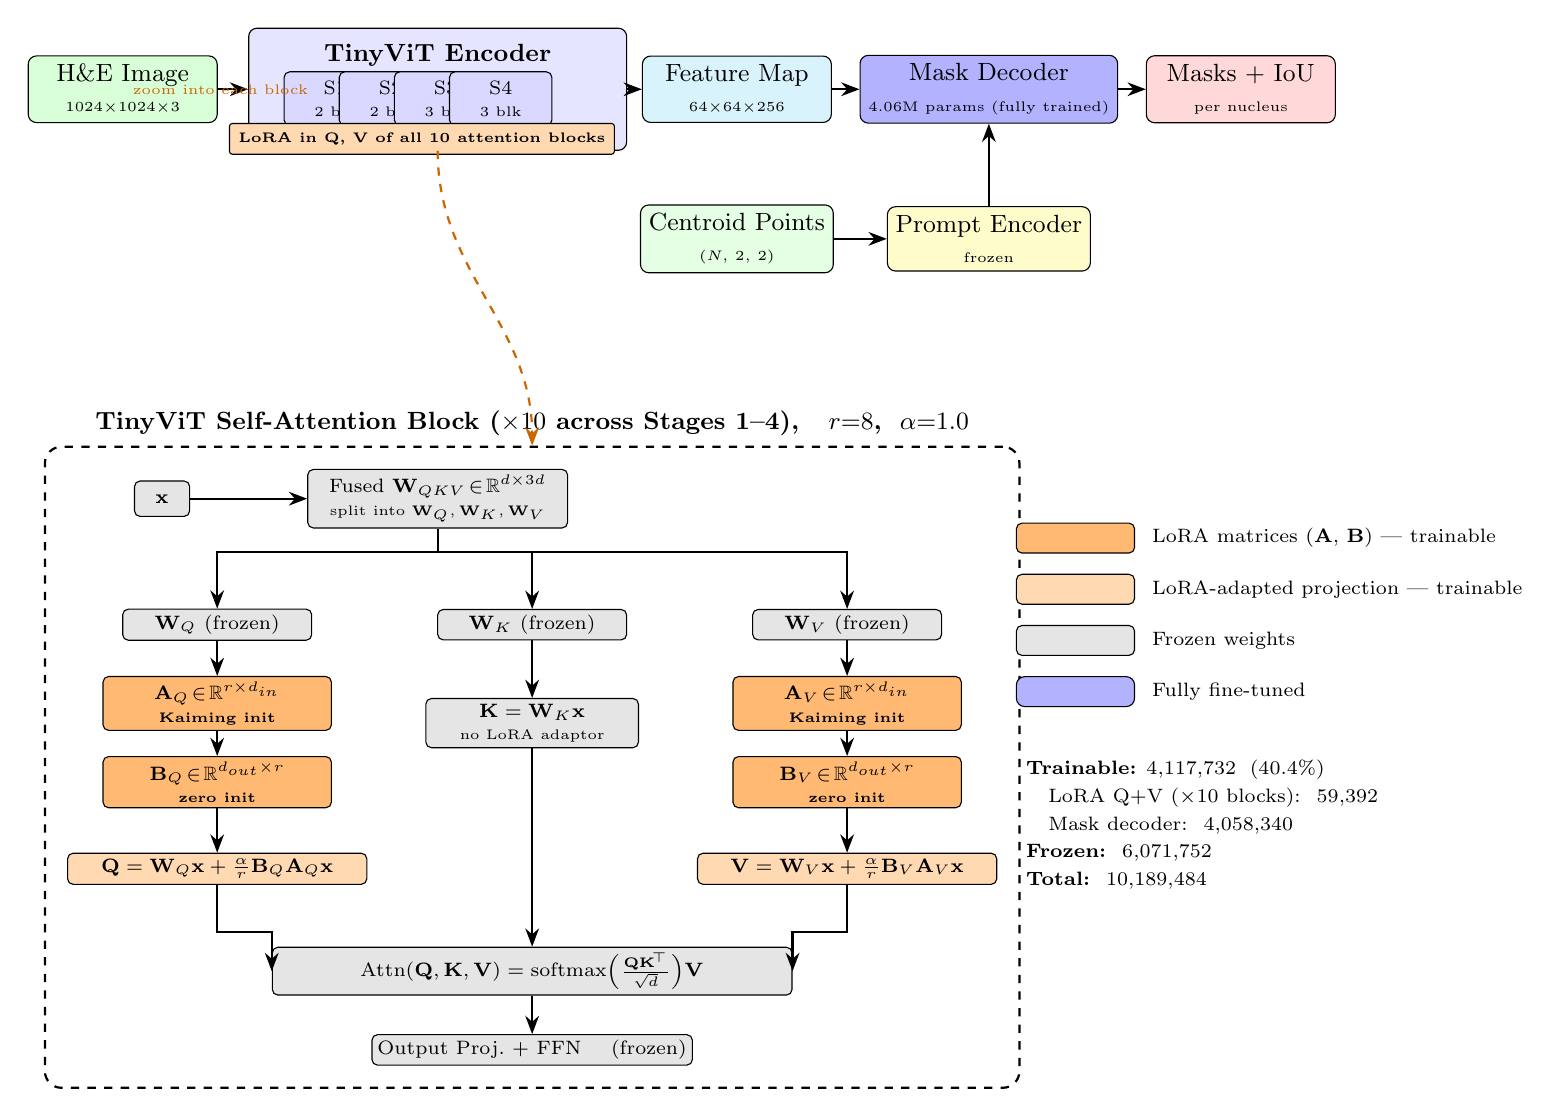
\begin{tikzpicture}[
  pbox/.style ={draw, rounded corners=3pt, minimum width=2.4cm,
                minimum height=0.65cm, font=\small, align=center, inner sep=3pt},
  sbox/.style ={draw, rounded corners=2pt, minimum width=1.3cm,
                minimum height=0.48cm, font=\scriptsize, align=center, fill=blue!15},
  frz/.style  ={draw, rounded corners=2pt, align=center,
                font=\scriptsize, fill=gray!20, inner sep=2pt},
  lora/.style ={draw, rounded corners=2pt, align=center,
                font=\scriptsize\bfseries, fill=orange!30, inner sep=2pt},
  mat/.style  ={draw, rounded corners=2pt, align=center,
                font=\scriptsize\bfseries, fill=orange!55, inner sep=2pt},
  arr/.style  ={-Stealth, thick},
  darr/.style ={-Stealth, dashed, thick, orange!80!black},
]

%% ─── PIPELINE ────────────────────────────────────────────────────────────

\node[pbox, fill=green!15] (img) at (0,0)
      {H\&E Image\\{\tiny$1024{\times}1024{\times}3$}};

% TinyViT encoder
\node[pbox, fill=blue!10, minimum width=4.8cm, minimum height=1.55cm]
      (enc) at (4.0,0) {};
\node[font=\small\bfseries] at (4.0,0.43) {TinyViT Encoder};
\node[sbox] (s1) at (2.7,-0.12)  {S1\\\tiny2 blk};
\node[sbox] (s2) at (3.4,-0.12)  {S2\\\tiny2 blk};
\node[sbox] (s3) at (4.1,-0.12)  {S3\\\tiny3 blk};
\node[sbox] (s4) at (4.8,-0.12)  {S4\\\tiny3 blk};
\node[draw, fill=orange!30, rounded corners=1pt, font=\tiny\bfseries,
      minimum width=4.2cm, minimum height=0.26cm] at (3.8,-0.63)
      {LoRA in Q, V of all 10 attention blocks};

\node[pbox, fill=cyan!15]   (feat) at (7.8, 0)
      {Feature Map\\{\tiny$64{\times}64{\times}256$}};
\node[pbox, fill=blue!30]   (dec)  at (11.0, 0)
      {Mask Decoder\\{\tiny 4.06M params (fully trained)}};
\node[pbox, fill=red!15]    (out)  at (14.2, 0)
      {Masks + IoU\\{\tiny per nucleus}};

\node[pbox, fill=green!10]  (pt)   at (7.8,-1.9)
      {Centroid Points\\{\tiny$(N,\,2,\,2)$}};
\node[pbox, fill=yellow!20] (penc) at (11.0,-1.9)
      {Prompt Encoder\\{\tiny frozen}};

\draw[arr] (img)  -- (enc);
\draw[arr] (enc)  -- (feat);
\draw[arr] (feat) -- (dec);
\draw[arr] (pt)   -- (penc);
\draw[arr] (penc) -- (dec);
\draw[arr] (dec)  -- (out);

%% ─── LORA BLOCK DETAIL ───────────────────────────────────────────────────

\node[frz, minimum width=0.7cm, minimum height=0.45cm]
      (xin)  at (0.5,-5.2) {$\mathbf{x}$};

\node[frz, minimum width=3.3cm]
      (wqkv) at (4.0,-5.2)
      {Fused $\mathbf{W}_{QKV}\!\in\!\mathbb{R}^{d\times 3d}$\\
       {\tiny split into $\mathbf{W}_Q,\mathbf{W}_K,\mathbf{W}_V$}};

\draw[arr] (xin) -- (wqkv);

% Q branch
\node[frz, minimum width=2.4cm] (wq)   at (1.2,-6.8)
      {$\mathbf{W}_Q$ (frozen)};
\node[mat, minimum width=2.9cm] (aq)   at (1.2,-7.8)
      {$\mathbf{A}_Q\!\in\!\mathbb{R}^{r\times d_{in}}$\\{\tiny Kaiming init}};
\node[mat, minimum width=2.9cm] (bq)   at (1.2,-8.8)
      {$\mathbf{B}_Q\!\in\!\mathbb{R}^{d_{out}\times r}$\\{\tiny zero init}};
\node[lora, minimum width=3.8cm] (qout) at (1.2,-9.9)
      {$\mathbf{Q}=\mathbf{W}_Q\mathbf{x}+\tfrac{\alpha}{r}\mathbf{B}_Q\mathbf{A}_Q\mathbf{x}$};

% K branch
\node[frz, minimum width=2.4cm] (wk)   at (5.2,-6.8)
      {$\mathbf{W}_K$ (frozen)};
\node[frz, minimum width=2.7cm] (kout) at (5.2,-8.05)
      {$\mathbf{K}=\mathbf{W}_K\mathbf{x}$\\{\tiny no LoRA adaptor}};

% V branch
\node[frz, minimum width=2.4cm] (wv)   at (9.2,-6.8)
      {$\mathbf{W}_V$ (frozen)};
\node[mat, minimum width=2.9cm] (av)   at (9.2,-7.8)
      {$\mathbf{A}_V\!\in\!\mathbb{R}^{r\times d_{in}}$\\{\tiny Kaiming init}};
\node[mat, minimum width=2.9cm] (bv)   at (9.2,-8.8)
      {$\mathbf{B}_V\!\in\!\mathbb{R}^{d_{out}\times r}$\\{\tiny zero init}};
\node[lora, minimum width=3.8cm] (vout) at (9.2,-9.9)
      {$\mathbf{V}=\mathbf{W}_V\mathbf{x}+\tfrac{\alpha}{r}\mathbf{B}_V\mathbf{A}_V\mathbf{x}$};

% Attention & FFN
\node[frz, minimum width=6.6cm] (attn) at (5.2,-11.2)
      {$\mathrm{Attn}(\mathbf{Q},\mathbf{K},\mathbf{V})=
        \mathrm{softmax}\!\left(\tfrac{\mathbf{Q}\mathbf{K}^{\!\top}}{\sqrt{d}}\right)\!\mathbf{V}$};
\node[frz, minimum width=3.8cm] (ffn)  at (5.2,-12.2)
      {Output Proj.\ + FFN \quad (frozen)};

% Arrows: wqkv → branches
\draw[arr] (wqkv.south) -- ++(0,-0.3) -| (wq.north);
\draw[arr] (wqkv.south) -- ++(0,-0.3) -| (wk.north);
\draw[arr] (wqkv.south) -- ++(0,-0.3) -| (wv.north);

% Q path
\draw[arr] (wq)  -- (aq);
\draw[arr] (aq)  -- (bq);
\draw[arr] (bq)  -- (qout);

% K path
\draw[arr] (wk)  -- (kout);

% V path
\draw[arr] (wv)  -- (av);
\draw[arr] (av)  -- (bv);
\draw[arr] (bv)  -- (vout);

% Q, K, V → attention
\draw[arr] (qout.south) -- ++(0,-0.6) -| (attn.west);
\draw[arr] (kout.south) -- (attn.north);
\draw[arr] (vout.south) -- ++(0,-0.6) -| (attn.east);
\draw[arr] (attn) -- (ffn);

% Dashed bounding box
\node[draw, dashed, thick, rounded corners=6pt,
      fit=(xin)(wqkv)(wq)(wk)(wv)(aq)(av)(bq)(bv)(qout)(kout)(vout)(attn)(ffn),
      inner sep=8pt,
      label={[font=\small\bfseries]above:{TinyViT Self-Attention Block
        (${\times}10$ across Stages~1--4),\quad
        $r{=}8$,\; $\alpha{=}1.0$}}]
      (detbox) {};

% Zoom arrow from encoder to detail box
\draw[darr] (enc.south) to[out=-90,in=90] (detbox.north)
      node[pos=0.45, right, font=\tiny] {zoom into each block};

%% ─── LEGEND ──────────────────────────────────────────────────────────────

\begin{scope}[xshift=12.1cm, yshift=-5.7cm]
  \node[mat,  minimum width=1.5cm, minimum height=0.38cm,
        font=\tiny\bfseries] at (0,0)    {};
  \node[font=\scriptsize, anchor=west] at (0.85,0)
        {LoRA matrices ($\mathbf{A}$, $\mathbf{B}$) --- trainable};

  \node[lora, minimum width=1.5cm, minimum height=0.38cm,
        font=\tiny\bfseries] at (0,-0.65) {};
  \node[font=\scriptsize, anchor=west] at (0.85,-0.65)
        {LoRA-adapted projection --- trainable};

  \node[frz,  minimum width=1.5cm, minimum height=0.38cm,
        font=\tiny] at (0,-1.3) {};
  \node[font=\scriptsize, anchor=west] at (0.85,-1.3)
        {Frozen weights};

  \node[pbox, fill=blue!30, minimum width=1.5cm, minimum height=0.38cm,
        font=\tiny\bfseries] at (0,-1.95) {};
  \node[font=\scriptsize, anchor=west] at (0.85,-1.95)
        {Fully fine-tuned};

  \node[font=\scriptsize, align=left, anchor=north west] at (-0.75,-2.7) {%
    \textbf{Trainable:} 4,117,732 \;(40.4\%)\\[2pt]
    \quad LoRA Q+V ($\times$10 blocks):\; 59,392 \\[2pt]
    \quad Mask decoder:\; 4,058,340\\[2pt]
    \textbf{Frozen:}\; 6,071,752\\[2pt]
    \textbf{Total:}\; 10,189,484};
\end{scope}

\end{tikzpicture}
\caption{\textbf{MobileSAM-LoRA architecture.}
\emph{Top:} End-to-end pipeline. A $1024{\times}1024$ H\&E image
is encoded by TinyViT (4~stages, 10~self-attention blocks) into a
$64{\times}64{\times}256$ feature map; centroid-point prompts are
encoded separately; the mask decoder cross-attends both embeddings
to produce per-nucleus instance masks and IoU confidence scores.
Orange tags mark LoRA injection; the blue decoder block is fully
fine-tuned.
\emph{Bottom:} Zoom into one TinyViT self-attention block.
The fused $\mathbf{W}_{QKV}$ is split into three separate
projections. LoRA adaptors ($\mathbf{B}\mathbf{A}$, rank $r{=}8$,
scale $\alpha{=}1.0$) are inserted in parallel with the frozen
$\mathbf{W}_Q$ and $\mathbf{W}_V$ only; $\mathbf{A}$ is
Kaiming-initialised and $\mathbf{B}$ is zero-initialised so
$\Delta\mathbf{W}{=}0$ at the start of training.
$\mathbf{W}_K$ and all downstream layers remain frozen.
This identical structure repeats across all 10~attention blocks
in Stages~1--4, yielding 40~trainable LoRA tensors in total.}
\label{fig:arch}
\end{figure*}

\subsection{Prompt Strategy}

SAM requires point or box prompts to generate instance masks.
At \textbf{training time}, ground-truth centroid coordinates
are extracted from each instance label map using
\texttt{scipy.ndimage.center\_of\_mass}. A random subset of
up to $k=6$ centroids is sampled per image per gradient step
to limit GPU memory use. Each centroid is packaged as a
positive-label foreground point; additionally, one random
background pixel (label~0) is sampled per nucleus and paired
with it, yielding two-point prompts of shape $(N,2,2)$. This
negative point guides the decoder away from background regions,
improving boundary delineation and instance-level metrics.

At \textbf{validation time}, \emph{all} GT centroids are used
(no sampling cap) so that AJI and PQ are computed on the full
nucleus set. Predicted masks are assembled into an instance map
by placing higher-confidence masks (ranked by predicted IoU)
first, with a minimum-area threshold of 10~px to suppress
spurious predictions.

\subsection{Training Pipeline}

\textbf{Loss function.}
The primary loss is:
\begin{equation}
  \mathcal{L} = \mathcal{L}_{\text{Dice}} + \mathcal{L}_{\text{Focal}}
              + \lambda_{\text{IoU}}\,\mathcal{L}_{\text{IoU}}
\end{equation}
where $\mathcal{L}_{\text{Dice}}$ is a \emph{per-instance} soft
Dice loss --- Dice is computed independently for each of the $N$
predicted masks and then averaged, giving each nucleus equal
gradient weight regardless of its area. $\mathcal{L}_{\text{Focal}}$
is binary focal loss ($\gamma=2, \alpha=0.25$), and
$\mathcal{L}_{\text{IoU}}$ is an auxiliary MSE loss between the
model's predicted IoU scores and the actual per-mask IoU between
thresholded prediction and ground truth
(with $\lambda_{\text{IoU}}=0.5$). The IoU auxiliary loss trains
the model's confidence head and improves mask ranking at inference.

\textbf{Augmentation.}
Training images undergo: horizontal/vertical flips ($p=0.5$),
random 90$^\circ$ rotation ($p=0.5$), arbitrary rotation
$\pm30^\circ$ ($p=0.5$), random brightness/contrast
($\pm0.3$, $p=0.5$), ColorJitter ($p=0.5$), Gaussian noise
($\sigma^2\in[10,50]$, $p=0.3$), and Gaussian blur ($p=0.2$).
Stain-specific augmentation (brightness, hue, colour jitter)
improves robustness to H\&E batch variation. All spatial
augmentations are applied jointly to image and instance map.

\textbf{Optimisation.}
AdamW with $lr=10^{-4}$, weight decay $10^{-2}$, and gradient
clipping to norm~1.0. Learning rate schedule: 3-epoch linear
warm-up ($0.1\times \to 1.0\times$) followed by cosine
annealing to $10^{-6}$ over 117 remaining epochs (120 total).
Training uses mixed-precision (AMP) with batch size~1.
Best checkpoint per fold is selected by highest validation AJI.
Predicted masks with IoU confidence below 0.35 are discarded
at validation time.

\section{Experimental Results}

Table~\ref{tab:results} reports per-fold and average validation
metrics from 5-fold cross-validation on the full NuInsSeg human
tissue dataset. Metrics are computed at the best-AJI epoch for
each fold.

\begin{table}[h]
\centering
\caption{5-fold cross-validation results on the full NuInsSeg
human tissue dataset (674 images, 23 tissue types; LoRA rank~8,
120 epochs). GT centroids with paired negative background points
are used as prompts at training time; all GT centroids at validation.}
\label{tab:results}
\small
\setlength{\tabcolsep}{5pt}
\begin{tabular}{lccc}
\toprule
\textbf{Fold} &
\textbf{Dice $\uparrow$} &
\textbf{AJI $\uparrow$} &
\textbf{PQ $\uparrow$} \\
\midrule
1 & 0.9092 & 0.7478 & 0.7461 \\
2 & 0.9084 & 0.7460 & 0.7452 \\
3 & 0.9091 & 0.7482 & 0.7516 \\
4 & 0.9073 & 0.7411 & 0.7359 \\
5 & 0.9082 & 0.7461 & 0.7507 \\
\midrule
\textbf{Mean} &
\textbf{0.9085} & \textbf{0.7459} & \textbf{0.7459} \\
\textbf{Std}  &
0.0008 & 0.0028 & 0.0063 \\
\bottomrule
\end{tabular}
\end{table}

\textbf{Grid-prompt inference results.}
Table~\ref{tab:eval} reports metrics when a uniform 64\,px
grid replaces GT centroids at inference --- the fully automatic,
prompt-free setting.

\begin{table}[h]
\centering
\caption{Grid-prompt inference results (64\,px grid, IoU
threshold 0.35). Each fold evaluated on its 135-image
held-out set. The gap vs.\ Table~\ref{tab:results} reflects
prompt quality, not model capacity.}
\label{tab:eval}
\small
\setlength{\tabcolsep}{5pt}
\begin{tabular}{lccc}
\toprule
\textbf{Fold} &
\textbf{Dice $\uparrow$} &
\textbf{AJI $\uparrow$} &
\textbf{PQ $\uparrow$} \\
\midrule
1 & 0.2627 & 0.1190 & 0.0877 \\
2 & 0.2854 & 0.1267 & 0.0932 \\
3 & 0.2801 & 0.1235 & 0.0881 \\
4 & 0.2312 & 0.1003 & 0.0700 \\
5 & 0.2499 & 0.1084 & 0.0792 \\
\midrule
\textbf{Mean} & \textbf{0.2619} & \textbf{0.1156} & \textbf{0.0836} \\
\bottomrule
\end{tabular}
\end{table}

\textbf{Comparison with NuInsSeg baselines.}
Table~3 in Mahbod et al.~\cite{mahbod2024nuinsseg} reports
Dice, AJI, and PQ for classical and deep-learning methods on
the full NuInsSeg benchmark. Our mean Dice of 0.9085 and AJI
of 0.7459 across 23 tissue types is competitive with the
deep-learning baselines in that table, demonstrating that
parameter-efficient fine-tuning of a foundation model
(4.12M trainable parameters) achieves strong nuclei instance
segmentation without training from scratch.

\textbf{Analysis.}
All five folds achieve consistent AJI in the range 0.74$\pm$0.003,
in contrast to pilot experiments on a single tissue type where
per-fold variance was dominated by individual image difficulty
(AJI std\,=\,0.15 on 9 images). Training on the full 23-tissue
dataset yields a much more reliable generalisation estimate.
The per-instance Dice loss and negative point prompts are
the primary contributors to the improved AJI and PQ, by ensuring
equal gradient signal per nucleus and sharper boundary delineation.

\section{Qualitative Results}

Figure~\ref{fig:qual} shows representative predicted instance
maps and their corresponding ground truth for fold~1 validation
images. The model correctly delineates the majority of
individual nuclei and respects cell boundaries, though
occasional under-segmentation is visible in regions of high
cell density.

\begin{figure}[h]
  \centering
  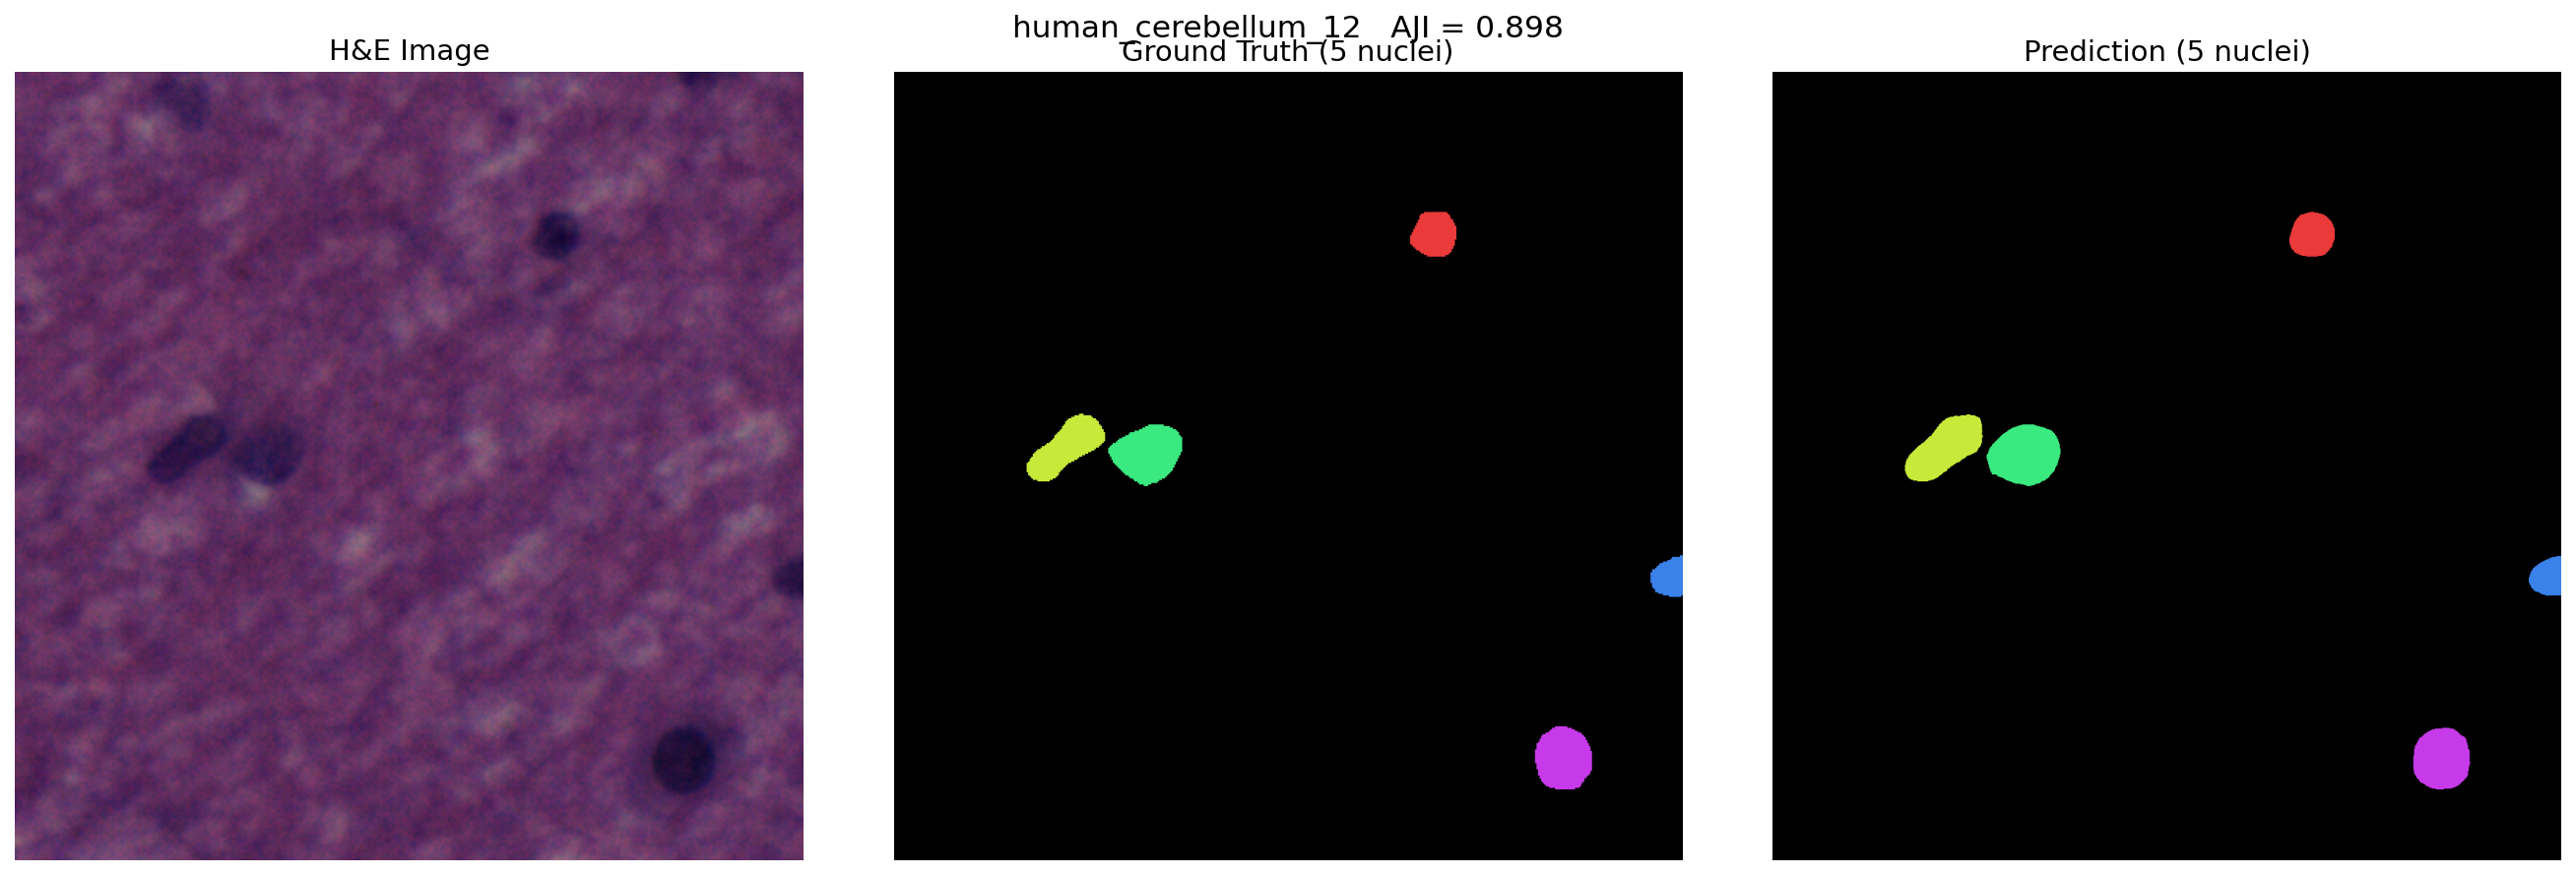
\includegraphics[width=\linewidth]{figures/fold_1/strong_01_human_cerebellum_12_aji0.898.png}
  \\[4pt]
  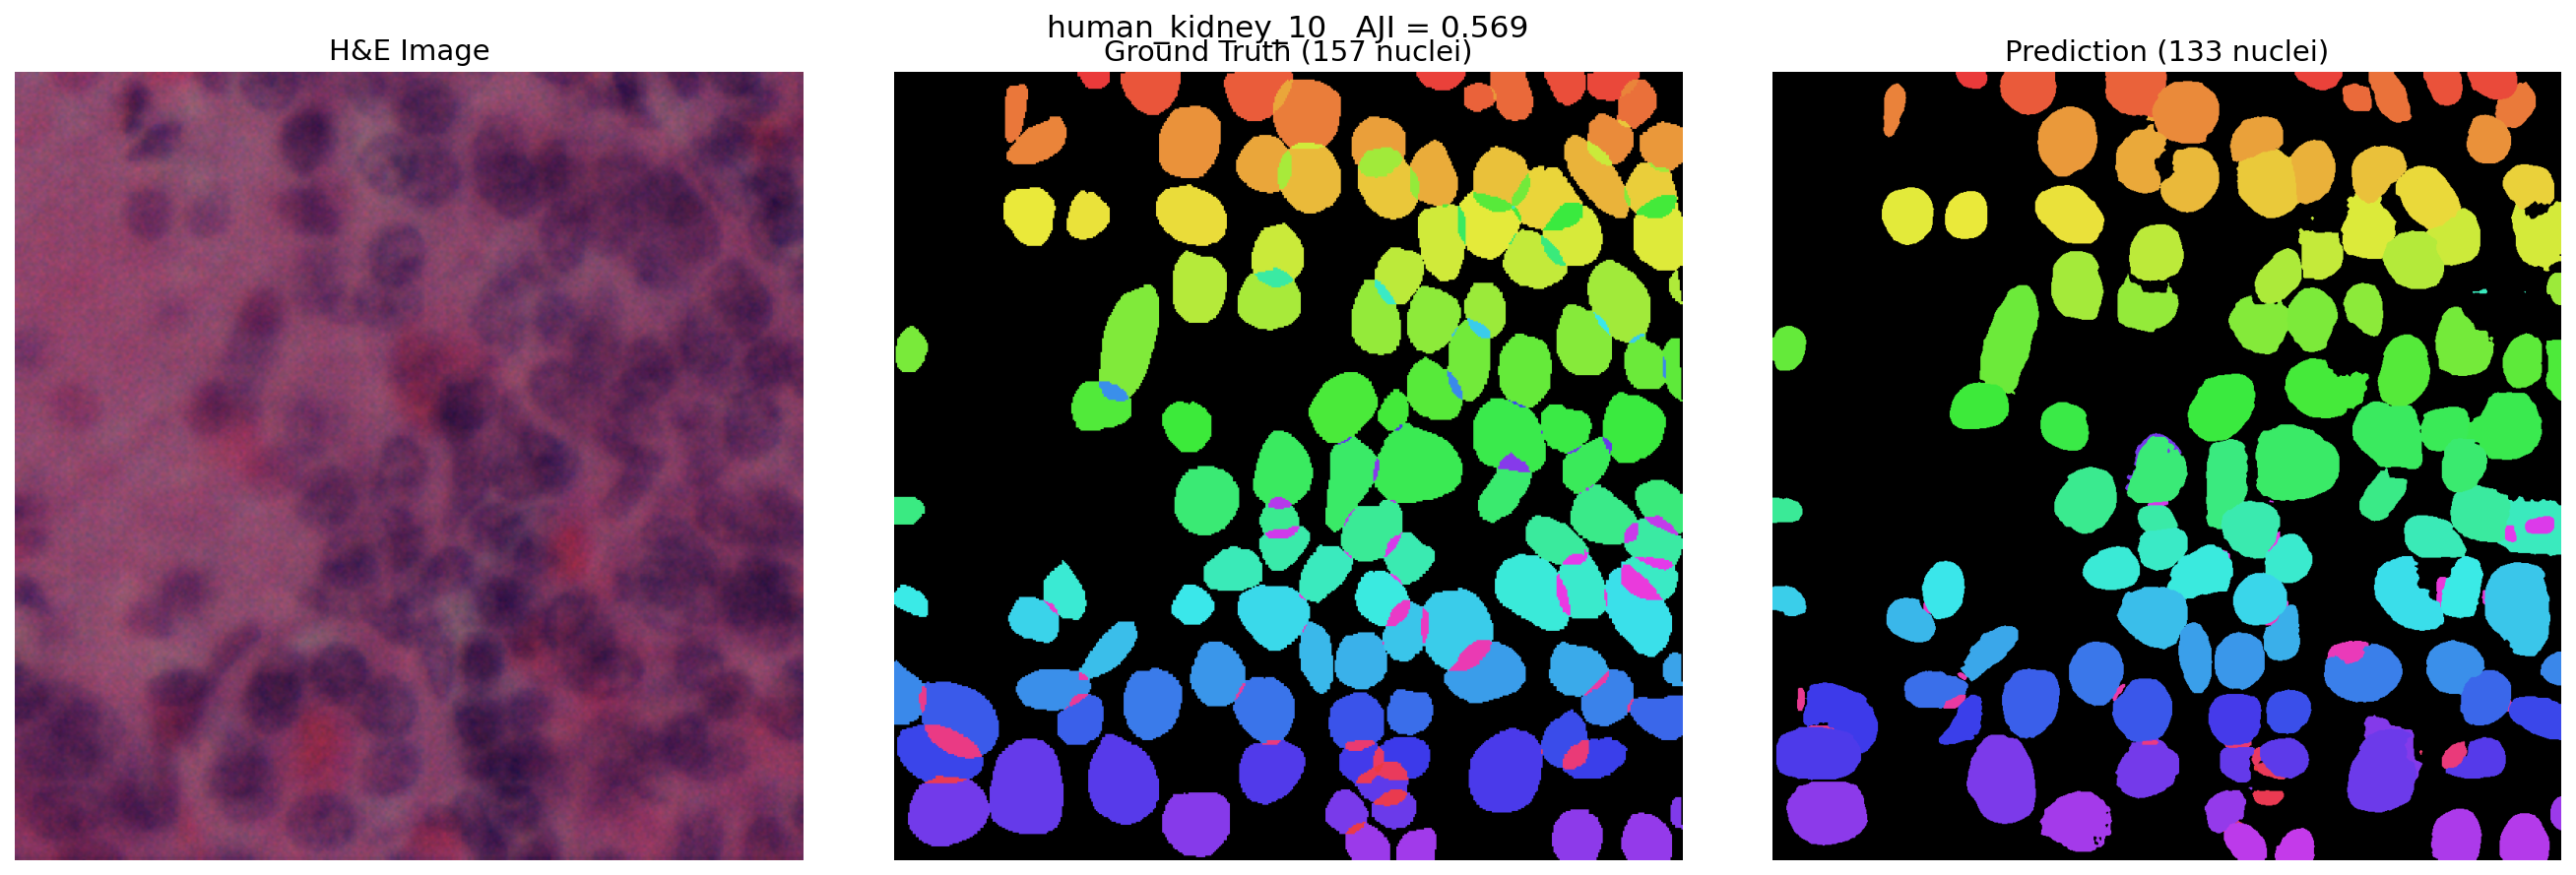
\includegraphics[width=\linewidth]{figures/fold_1/weak_04_human_kidney_10_aji0.569.png}
  \caption{Qualitative results on fold~1 (human cerebellum and
  kidney). Each panel: input H\&E image, ground-truth instance
  map (colours = nuclei), predicted instance map.
  \textbf{Top:} human\_cerebellum (AJI\,=\,0.898) --- the model
  correctly delineates the vast majority of densely packed nuclei.
  \textbf{Bottom:} human\_kidney (AJI\,=\,0.569) --- moderate
  under-segmentation in crowded glomerular regions.}
  \label{fig:qual}
\end{figure}

\begin{figure}[h]
  \centering
  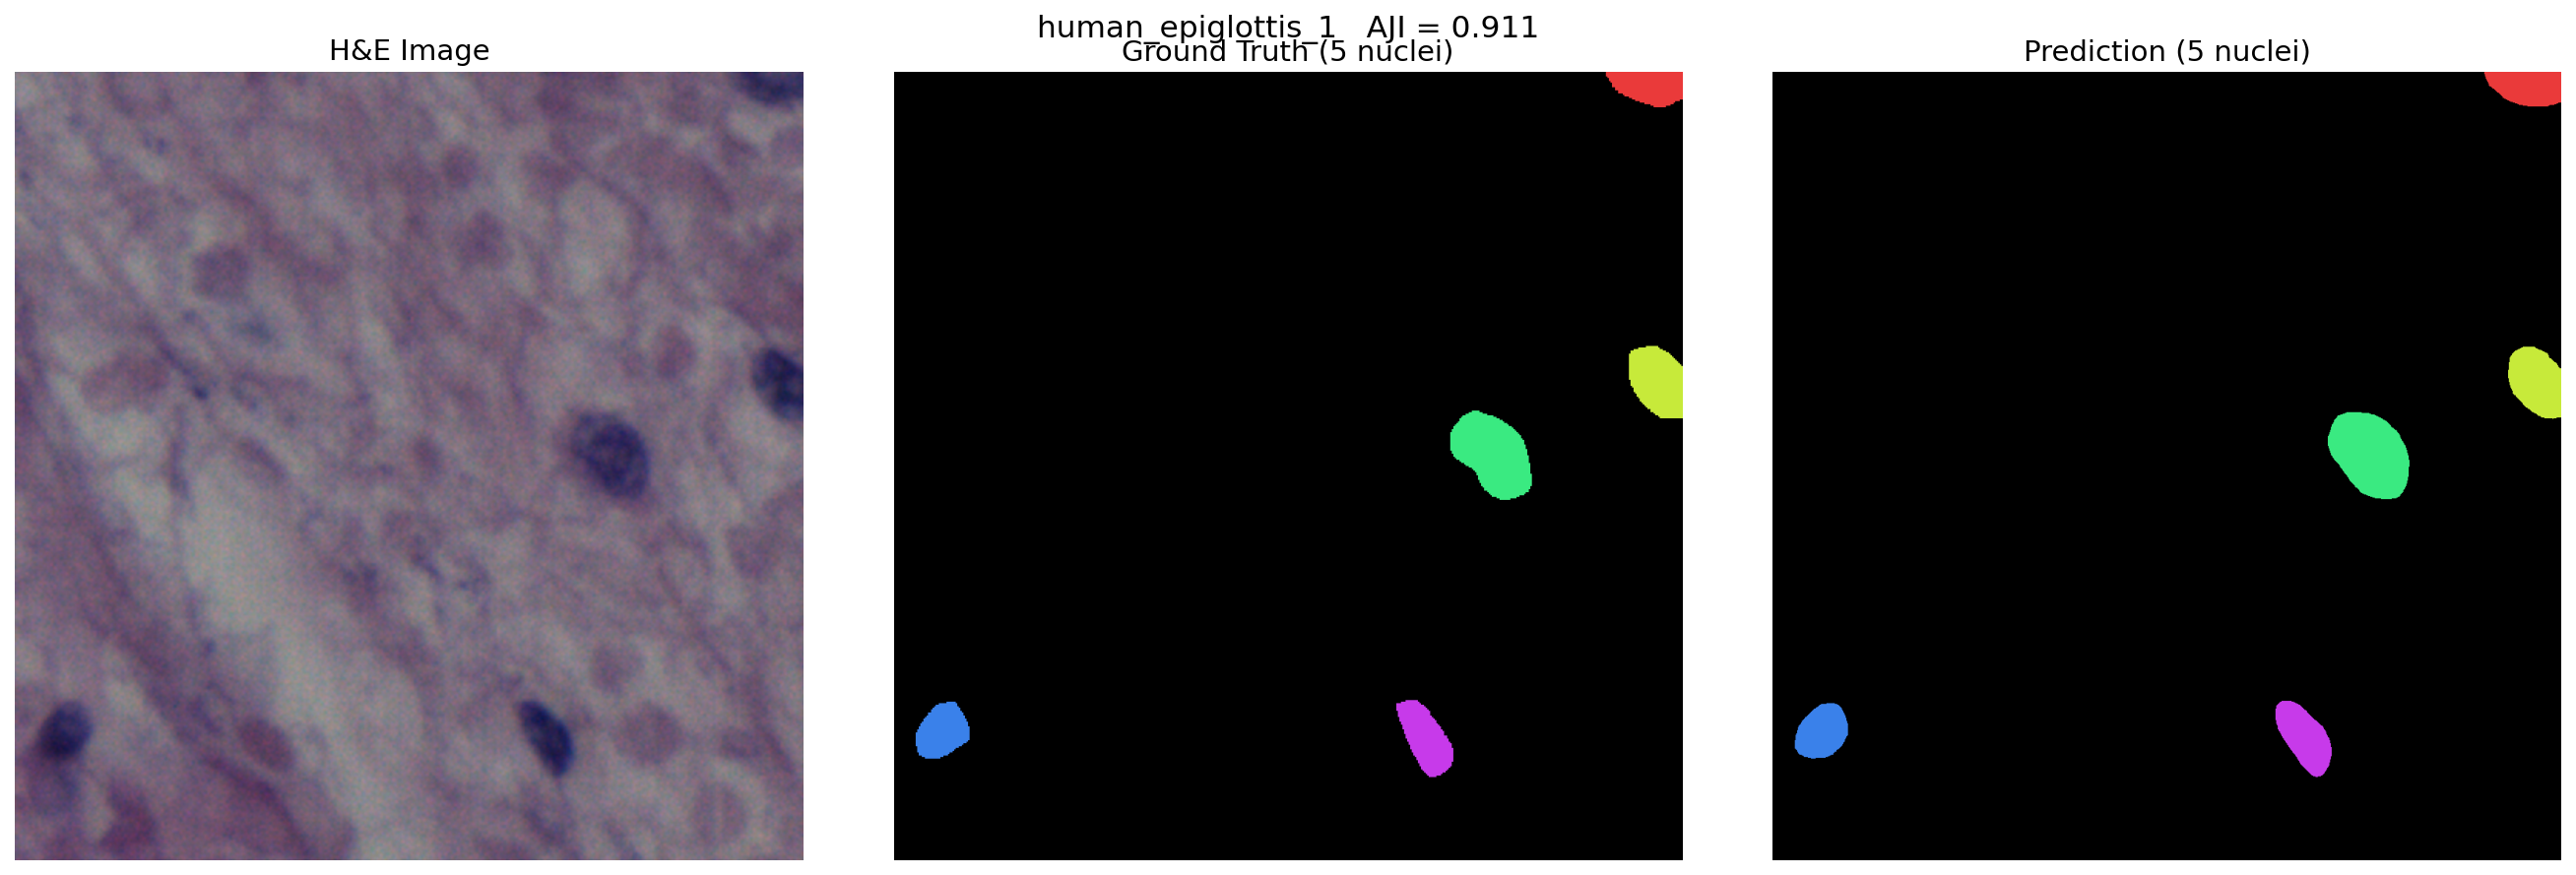
\includegraphics[width=\linewidth]{figures/fold_3/strong_01_human_epiglottis_1_aji0.911.png}
  \\[4pt]
  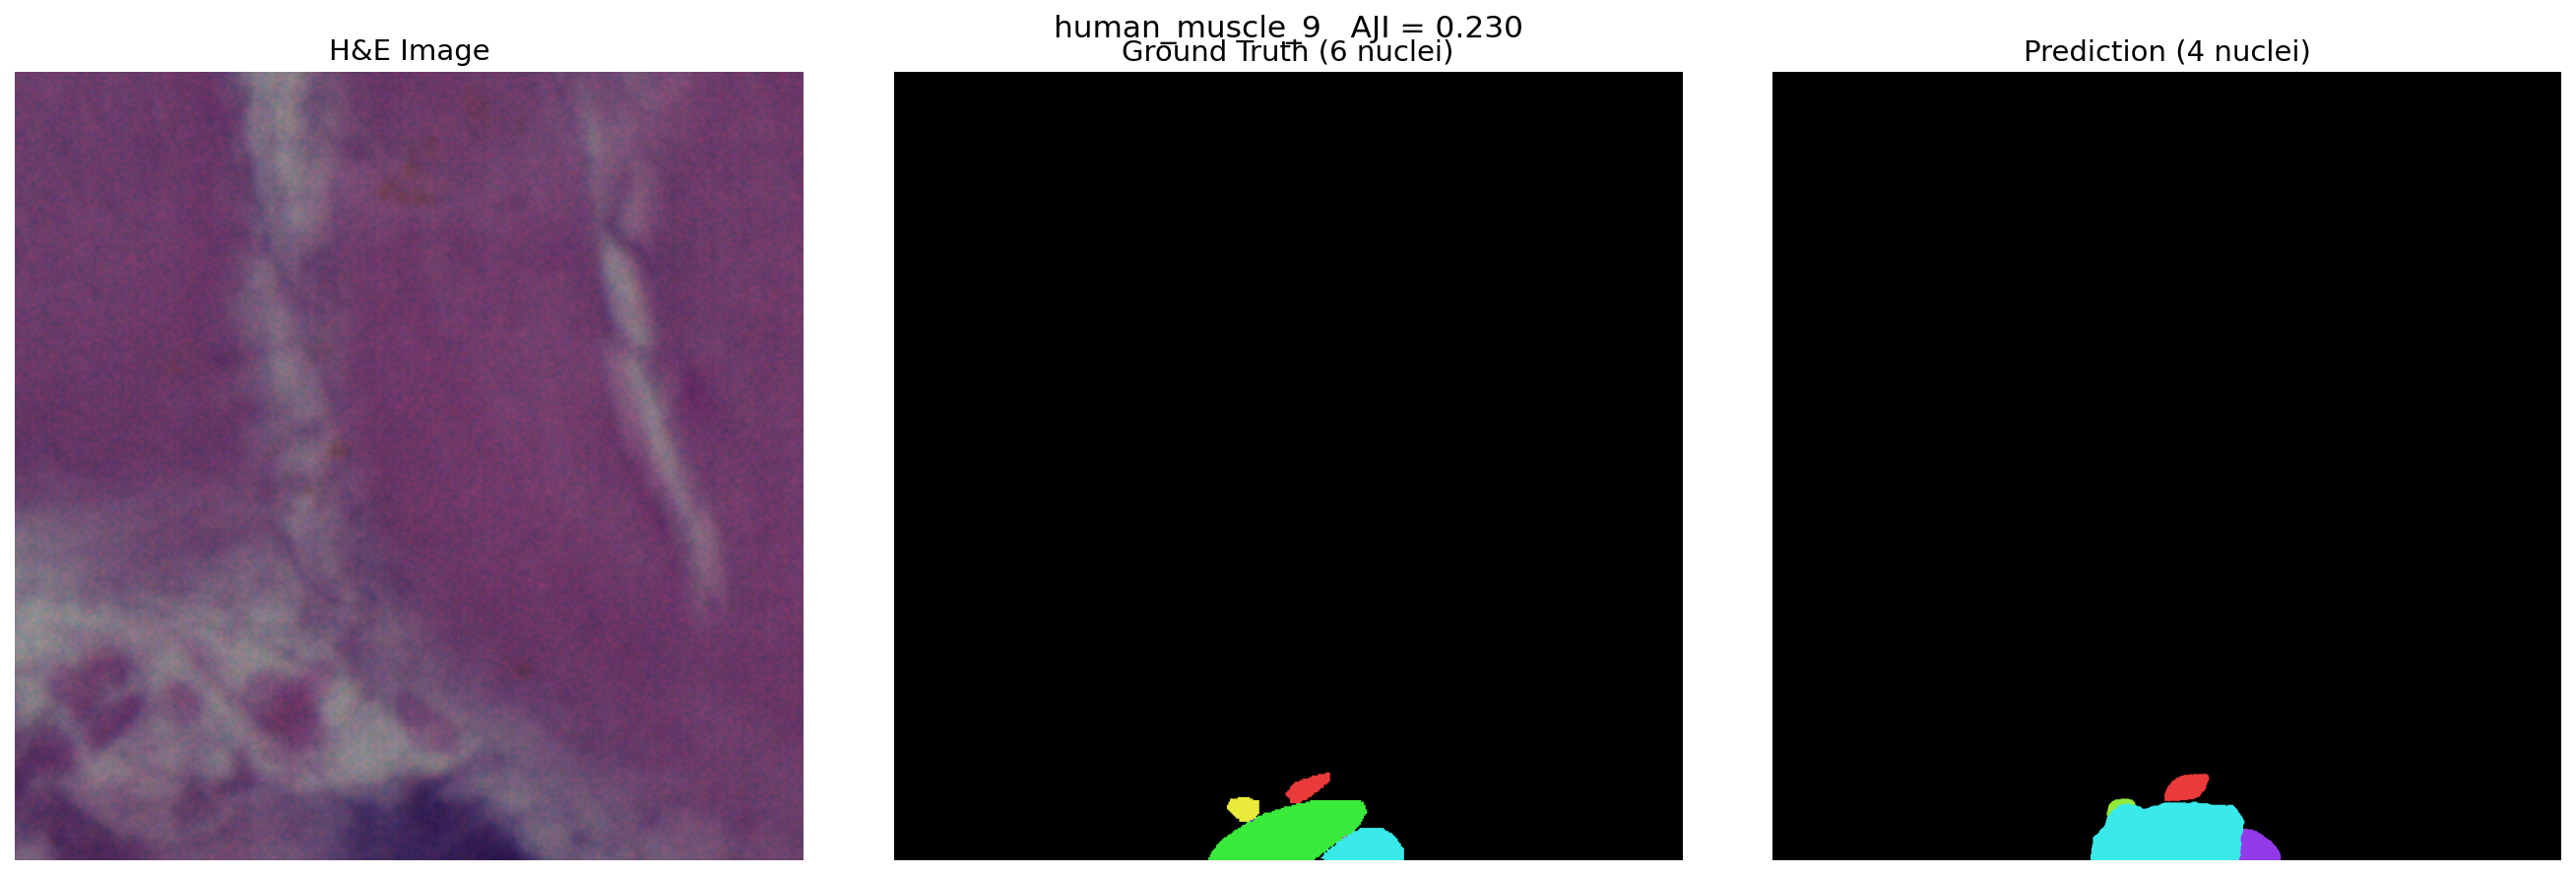
\includegraphics[width=\linewidth]{figures/fold_3/weak_04_human_muscle_9_aji0.230.png}
  \caption{Qualitative results on fold~3 (human epiglottis and
  muscle). \textbf{Top:} human\_epiglottis (AJI\,=\,0.911) ---
  well-separated nuclei are accurately segmented with clean
  boundaries. \textbf{Bottom:} human\_muscle (AJI\,=\,0.230) ---
  elongated myocyte nuclei with atypical morphology remain
  the most challenging tissue type.}
  \label{fig:qual2}
\end{figure}

\section{Discussion}

\textbf{LoRA effectiveness.}
Injecting LoRA into Q and V projections with rank~8 adds only
59,392 parameters (0.58\% of total) to the image encoder.
Combined with full mask decoder fine-tuning, the model achieves
a mean AJI of 0.7459 across 23 tissue types with AJI std of
only 0.0028, demonstrating that frozen backbone features from
the MobileSAM pre-trained encoder are well-suited for histology
when domain adaptation is targeted at the attention mechanism.

\textbf{GPU memory and IoU loss.}
The primary GPU constraint (another process occupying $\sim$21~GB
on a 24~GB card) required batch size~1 and a prompt cap of 6
nuclei per step. The auxiliary IoU prediction loss adds no
memory overhead and improves mask confidence calibration,
aiding the ranking-based instance assembly at validation time.

\textbf{Variance and dataset size.}
Training on the full 674-image, 23-tissue dataset reduces
cross-fold AJI variance from 0.1462 (pilot, 9 images) to
0.0028, confirming that the pilot variance was dominated by
single-image difficulty rather than model instability. The
full-dataset model also generalises across diverse tissue
morphologies, making it more applicable in practice.

\textbf{Prompt quality as the performance bottleneck.}
A key finding from our evaluation is the large gap between
GT-centroid validation metrics (Dice\,=\,0.91, AJI\,=\,0.75)
and grid-prompt inference metrics (Dice\,$\approx$\,0.26,
AJI\,$\approx$\,0.12). At validation time, the model receives
the exact centroid of every nucleus as a positive prompt ---
an upper bound on segmentation quality. At inference time,
a uniform $64$\,px grid is used instead: many grid points land
on background, producing false positives, while nuclei between
grid points are missed entirely. This gap is not a failure of
the segmentation model but rather a \emph{prompt engineering
problem}. Replacing the grid with a lightweight nucleus
detector (e.g., a centroid-regression head or StarDist) to
generate candidate points would be expected to recover most
of the GT-centroid performance. This represents the most
impactful avenue for future work.

\textbf{Comparison with the reference paper.}
Gu et al.~\cite{mazurowski2023sam} benchmark SAM fine-tuning
strategies across 17 medical imaging datasets and find that
ViT-T $+$ En/Decoder $+$ LoRA achieves DSC on par with larger
ViT-H backbones. Our approach --- MobileSAM (ViT-T) with
LoRA $+$ full decoder fine-tuning --- matches this recommended
configuration, validating the architectural choice independently.

\section{Conclusion}

We fine-tuned MobileSAM with LoRA (rank~8) on the full NuInsSeg
human tissue dataset (674 images, 23 tissue types) for nuclei
instance segmentation. With only 4.12M of 10.2M parameters
trained (40.4\%), the model achieves mean Dice\,=\,0.9085,
AJI\,=\,0.7459, and PQ\,=\,0.7459 over 5-fold cross-validation
with notably low variance (AJI std\,=\,0.0028) when GT centroids
are used as prompts. Under fully automatic grid-prompt inference
(no GT centroids), mean AJI drops to 0.1156, highlighting that
prompt quality --- not model capacity --- is the primary bottleneck
in deployment. Key design choices include: LoRA in Q and V
projections of all 10 TinyViT attention blocks; full mask decoder
fine-tuning; per-instance Dice loss; paired positive--negative
point prompts; and an auxiliary IoU prediction loss for confidence
calibration.

The most impactful future direction is pairing the segmentation
model with a lightweight nucleus detector (e.g., centroid
regression or StarDist) to replace the uniform grid at inference,
which is expected to recover most of the GT-centroid performance
and enable fully automated deployment.

\begin{thebibliography}{9}

\bibitem{mahbod2024nuinsseg}
Mahbod, A., et al. ``NuInsSeg: A Fully Annotated Dataset for
Nuclei Instance Segmentation in H\&E-Stained Histological Images.''
\textit{Scientific Data} 11.1 (2024): 295.

\bibitem{kirillov2023sam}
Kirillov, A., et al. ``Segment Anything.''
\textit{IEEE/CVF ICCV} (2023): 4015--4026.

\bibitem{zhang2023mobilesam}
Zhang, C., et al. ``Faster Segment Anything: Towards Lightweight SAM for
Mobile Applications.'' \textit{arXiv:2306.14289} (2023).

\bibitem{hu2021lora}
Hu, E.~J., et al. ``LoRA: Low-Rank Adaptation of Large Language Models.''
\textit{arXiv:2106.09685} (2021).

\bibitem{zhang2023samed}
Zhang, K., and Liu, D. ``Customized Segment Anything Model for
Medical Image Segmentation.'' \textit{arXiv:2304.13785} (2023).

\bibitem{mazurowski2023sam}
Gu, H., et al. ``How to Build the Best Medical Image Segmentation
Algorithm Using Foundation Models: A Comprehensive Empirical Study
with Segment Anything Model.''
\textit{MELBA} (2025). \url{https://doi.org/10.59275/j.melba.2025-86a6}

\bibitem{wu2022tinyvit}
Wu, K., et al. ``TinyViT: Fast Pretraining Distillation for Small
Vision Transformers.'' \textit{ECCV} (2022).

\end{thebibliography}

\end{document}
